%%==================================================
%% diss.tex for SJTU Bachelor Thesis
%% based on CASthesis
%% version: 0.3a
%% Encoding: UTF-8
%%==================================================

% 字号选项: c5size 五号(默认) cs4size 小四
% 双面打印(注意字号设置)
%\documentclass[cs4size, a4paper, twoside]{sjtuthesis} 
% 单面打印(注意字号设置)
\documentclass[cs4size, a4paer, oneside, openany]{sjtuthesis} 


% \usepackage[sectionbib]{chapterbib}%每章都用参考文献
\usepackage{setspace}
\newboolean{DOIT}
\setboolean{DOIT}{false}%编译某些只想自己看的内容,编译true,否则false

%% 行距缩放因子(x倍字号)
\renewcommand{\baselinestretch}{1.3}

% 设置图形文件的搜索路径
\graphicspath{{figure/}{figures/}{logo/}{logos/}{graph/}{graphs}}

%%========================================
%% 在sjtuthesis.cls中定义的有用命令
%%========================================
% \cndash 中文破折号
% 数学常量
% \me 对数常数e
% \mi 虚数单位i
% \mj 虚数单位j
% \dif 直立的微分算符d为直立体。
% 可伸长的数学箭头、等号
% \myRightarrow{}{}
% \myLeftarrow{}{}
% \myBioarrow{}{}
% \myLongEqual{}{}
% 参考文献
% \upcite{} 上标引用
%%========================================


\begin{document}

%%%%%%%%%%%%%%%%%%%%%%%%%%%%%% 
%% 封面
%%%%%%%%%%%%%%%%%%%%%%%%%%%%%% 

% 中文封面内容(关注内容而不是形式)
\title{上海交通大学学士学位论文~\XeTeX/\LaTeX~模板~}
\author{李\quad{}四}
\advisor{张三教授}
\degree{学士}
\defenddate{2010年1月16日}
\school{上海交通大学}
\institute{理学院物理系}
\studentnumber{0010900990}
\major{物理系}

% 英文封面内容(关注内容而不是表现形式)
\englishtitle{\XeTeX/\LaTeX\, Template for SJTU Bachelor Degree Thesis \version}
\englishauthor{\textsc{Si Li}}
\englishadvisor{Prof. \textsc{San Zhang}}
\englishschool{Shanghai Jiao Tong University}
\englishinstitute{\textsc{Depart of XXX, School of XXX} \\
  \textsc{Shanghai Jiao Tong University} \\
  \textsc{Shanghai, P.R.China}}
\englishdegree{Bachelor}
\englishmajor{Physics}
\englishdate{Jan. 16th, 2010}

% 封面
\maketitle

% 英文封面
\makeenglishtitle

% 论文原创性声明和使用授权
\makeDeclareOriginal
\makeDeclareAuthorization

%%%%%%%%%%%%%%%%%%%%%%%%%%%%%% 
%% 前言
%%%%%%%%%%%%%%%%%%%%%%%%%%%%%% 
\frontmatter

% 摘要
%%==================================================
%% abstract.tex for SJTU Bachelor Thesis
%% version: 0.5.2
%% Encoding: UTF-8
%%==================================================

\begin{abstract}

学术搜索是指针对目前学术论文数据量十分巨大,难以直接获取所需要的文献的情况下,在现有会议论文数据中建立合适的索引和联系,以结构化的信息方便查找选择。类似传统搜索引擎,为用户提供关键字或分类查找等方便的搜索方式。

而与传统搜索引擎使用者不同的是,学术搜索引擎使用者往往需要对整个领域有一个较为宏观的掌握才能够比较有效的使用搜索功能查找所需要的文献。而在同一会议中发表的论文之间,往往具有较强的相关性。但即使在一个特定领域,也存在复数个会议。如何在会议之间进行论文的推荐就是比较困难的问题。目前国内外的这一领域里,均缺少比较深入的研究和完善的解决方案。即使是在大数据十分火热的现今,对于学术大数据的特殊研究,特别是会议之间的研究获得的关注并不多。而对于很多研究者来说,对于某个会议的论文的研究,或者是同一领域内数个会议之间论文的比较,会带来对研究领域的 比较清晰和完备的认识,对研究带来收获。

在现有的学术论文数据基础上,主要考虑利用会议之间文章的相似度来定义会议之间的关系,基于各种自然语言处理方法,例如词嵌入以及神经网络语言模型等NLP方法来对文章进行分析,在辅助以例如引用以及作者之间关系等信息,来实现协同过滤的推荐方法。

  \keywords{学术搜索,大数据,词嵌入, NLP, 推荐系统}
\end{abstract}

\begin{englishabstract}

The academic search refers to deal with the large amount of academic papers, 

  \englishkeywords{\large acadamic search, BigData, word embedding, NLP, recommendation system}
\end{englishabstract}


% 目录
\tableofcontents
% 表格索引
\listoftables
% 插图索引
\listoffigures

% \addcontentsline{toc}{chapter}{\listfigurename} %将表格索引加入全文目录
% \addcontentsline{toc}{chapter}{\listtablename}  %将图索引加入全文目录

% 主要符号、缩略词对照表
% %%==================================================
%% symbol.tex for SJTU Bachelor Thesis
%% version: 0.5.2
%% Encoding: UTF-8
%%==================================================

\chapter{主要符号对照表}
\label{chap:symb}
\begin{tabular}{ll}

 \hspace{2em}$\epsilon$       & \hspace{5em}介电常数 \\
 \hspace{2em}$\mu$ \qquad     & \hspace{5em}磁导率 \\
  \hspace{2em}$\epsilon$       & \hspace{5em}介电常数 \\
 \hspace{2em}$\mu$ \qquad     & \hspace{5em}磁导率 \\
 \hspace{2em}$\epsilon$       & \hspace{5em}介电常数 \\
 \hspace{2em}$\mu$ \qquad     & \hspace{5em}磁导率 \\
 \hspace{2em}$\epsilon$       & \hspace{5em}介电常数 \\
 \hspace{2em}$\mu$ \qquad     & \hspace{5em}磁导率 \\


\end{tabular}


%%%%%%%%%%%%%%%%%%%%%%%%%%%%%% 
%% 正文
%%%%%%%%%%%%%%%%%%%%%%%%%%%%%% 
\mainmatter


%% 各章正文内容
%%==========================
%% chapter01.tex for SJTU Bachelor Thesis
%% version: 0.5.2
%% Encoding: UTF-8
%%==================================================

%\bibliographystyle{sjtu2} %[此处用于每章都生产参考文献]
\chapter{绪论}
\label{chap:introduction}

\section{学术搜索现状简介}
\label{sec:academic-intro}

网络信息时代下,各个学科的学术研究成果的交流自然而然变得更加频繁且不可或缺.其中在我们日常研究生活中最为经常应用到的部分就是灌注了其他研究者智慧果实和研究成果的学术论文.获取一篇想要阅读的论文通常需要自费购买或者依靠于对应的学术机构集体购买.例如IEEE的数据库\footnote{\url{http://ieeexplore.ieee.org}}以及国内的中国知网\footnote{\url{http://cnki.net}}.当然也有类似arXiv\footnote{\url{https://arxiv.org}}的网站可以免费阅读下载上面的论文. 然而这些数据库的问题在于其中存储的论文数据相互之间几乎没有交集.导致如果要寻找某一篇论文有时候必须遍历数个数据库才能找到具体想要的论文.这样的行为明显增加了学术研究中不必要的时间开销.而类似的情况以前也曾经出现过,那就是在互联网的发展的早期,各个网站之间并不完全相通,缺乏一个合适的流量引导的工具导致网络的相对闭塞.而门户网站以至于之后的搜索引擎的出现正是填补了这个空缺,让整个网络真正的互相连接起来了,也方便了在互联网上浏览的所有用户.而在网络中的学术论文这个领域,相对应出现的工具就是学术搜索引擎了.

在当今世界上,被应用得比较广泛,使用者数量比较多的学术搜索引擎应该要数美国Google公司开发的Google Scholar网站\footnote{\url{https://scholar.google.com}}.这个网站也是目前公开的,数据量最大,最方便的学术搜索引擎.这个搜索引擎的使用方式和普通的网站搜索引擎类似.支持按照关键词搜索,通过作者检索,通过高级搜索进行更加精确地搜索等功能\cite{夏旭2006基于}. Google Scholar也提供了学术论文作者的个人资料页面,其中可以看到该作者相关的很多信息,包括按年份划分的被引用数以及一些统计数据等.例如 \textbf{h-index},意义是被引用数超过该数字次数的文章数.从这些个人页面也可以很快地获得对此人研究成果的大致认知.可以说也从侧面加强了网站整体的功能性以及易用性.

与Google Scholar相似的,还有微软公司的微软学术搜索\footnote{\url{http://cn.bing.com/academic}}.是由微软亚洲研究院(MSRA)开发的免费学术搜索引擎。特点是使用了对象级别的信息检索途经,可以通过微软自己的数据库来找到某个学术领域内的领先的研究者和顶尖的会议和期刊,甚至还可以研究领域兴盛和发展的具体过程.还可以用来发现一些学术研究学科内的研究热点和正在上升期的学术新星等.虽然这个搜索引擎目前主要收录了与计算机科学和信息科学相关的学术数据,但这些更为高级的应用功能无疑是对于用户的使用体验有很大提高的.

除了这些国外公司开发的学术搜索引擎以外,国内也有高校开发出自己的学术搜索引擎,例如清华大学的AMiner\footnote{\url{https://aminer.org}}和上海交通大学的Acemap\footnote{\url{http://acemap.sjtu.edu.cn}}. 这些高校搜索引擎的特点是虽然数据量无法和Google Scholar那样的大体量比肩,但开发者更注重用户在使用学术搜索引擎时可能需要的一些个性化的功能.例如Acemap之中,用户可以通过可视化的方式,由大及小很轻松的选择出自己感兴趣的学术研究领域,来检索其中的论文.更可以通过合作者地图,学术机构地图等方式来贴合各种个性化的需求,来提高寻找所需要的学术论文的效率.


\section{系统简介}
\label{sec:nlp-intro}

由于在实际的学术研究中,相对于关注某个知名研究者或者研究机构的研究成果,我们往往会更加关注某一个领域的过往以及最新的研究成果也即是在该领域发表的学术论文.而且不同的人关注的领域往往并不会宽泛到某个一级学科甚至于二级学科,而是具体到某个很细分的方向.例如对于同样是关注机器学习这个领域的研究者,有些人关注的重点在于监督学习而有些人则会对非监督学习更为感兴趣.还有现在大火的增强学习,也是一个截然不同的领域.更进一步地,在相似的一些算法上,也有不同的侧重点在.这样就给我们在寻找一系列感兴趣的论文时增加了难度.仅仅依靠几个关键词无法很好的找到所需要的论文,更无法发现一些提出的崭新的思想和概念.而通过作者和合作者甚至于引用关系来检索也有很大的局限性,因为每个研究者的研究兴趣和方向也是会随着时间的变化而有相应的变化,无法仅仅通过锁定数个研究者来获得感兴趣的方向和领域的论文.很自然地,我们就产生了一个想法,如何通过现有的数据,来改善我们的学术搜索使用的体验,来更好的去切合我们去查找某个细分领域内所有优质论文的需求呢?

这乍一看是一个并没有表面上那么简单的想法.论文的思想和方向无法简单地通过数个关键词来定义.而具体涉及到论文的内容,要通过自然语言处理的方法来直接进行文本分类,来进一步地将我们所寻找的相似领域的论文来划分到一起,先不提其效果比较难以检验,学术论文作为研究者的思维结晶和学术成果,作为文本,它的单位信息量是大于我们常见的新闻,小说等文本类型的.而且论文文本之中结构也十分复杂,为了能够很好地将自己的研究成果向其他研究者阐述清楚,研究者们往往需要在学术论文之中附上大量的图标,数据,算法.这些并不标准的部分也增加了分析学术论文整个文本的难度.目前为止,有关于学术论文文本分类的研究比较少,想必也有这个方面的原因.所幸这个想法能够很自然地落到实处,通过自然语言处理方法来进行对应的学术论文分类并不是一个非常糟糕的选择.但具体应用到学术论文上时,我们考虑采取一些其他的手段来辅助我们的分类.

首先考虑到学术论文的特殊性在于其结构化较为明显,大部分发表的学术论文,基本上都包含了摘要,绪论,正文等几个部分.这也体现了学术论文与其他文本的区别的一点在于其作者都是经过了充分训练的科学工作者,其整体结构的严谨性自然能够得到保证.其次则是学术论文大多通过会议和期刊来发表.我们很自然地想到,在学术论文从写作到投稿这一过程中,研究者对于投稿的期刊和会议的选择,其实就是一次人为的标签行为.因为不同的期刊和会议,所接受的论文的研究主题和范围都是有所限定的.虽然有时候会随着时间的经过,世界上研究热点的变化而稍有变化,但依然能作为一个判定地依据.特别是学术会议,作为一个有时效性的活动,其中发表的学术论文的选题和方向通常都具有很强的时代性和针对性.与此相对的是许多期刊因为是长期发表的刊物,其内容受时间和时代的影响就比较明显.任何一个期刊里刊登在2016年的文章和2006年的文章关注的热点肯定是截然不同的.很显然,与其直接研究学术论文文本的分类,研究学术会议整体之间的关系,再通过相似的会议来进行学术论文的推荐就是一个比较容易且高效的方法.

那么对于一个了解数据挖掘的人来说,这个问题就集中到如何去在机器能够认识的领域内去定义一个学术会议了,简单地来说就是如何对学术会议去做特征提取.这时候又有一个很自然的想法,既然学术会议是其中学术论文的一个隐含的特征,如果我们把学术会议看做是学术论文的集合,那么我们显然可以通过其中包含的学术论文反过来定义会议本身.如何定义一篇学术论文呢?常见的文本特征抽取的方法有从简单的词频,\textbf{TF-IDF}到\textbf{N-gram}算法,模拟退火算法等较为复杂的方法.这里我们考虑到我们最终的目的在于理清学术会议之间一个相对的关系,注重的是相对.所以我采取了具有很好线性特征的Word2vec\cite{mikolov2013distributed,mikolov2013efficient}来实现最终的文本向量化.

具体的做法是利用单层的神经网络语言模型\textbf{Skip-gram}来训练词向量$\mathbf{V}_{word}$,再将训练好的词向量进行聚类.利用聚类来对文本向量化.聚类算法也有很多中选择,包括层次化聚类算法,划分式聚类算法以及基于网格和密度的聚类算法等\cite{孙吉贵2008聚类算法研究},这里我们选择使用划分式聚类算法中的\textbf{K-Means}算法来进行聚类.经过聚类之后的词向量,每个类型都代表了学术论文中比较接近的一类词语,这时候我们只需要简单的统计出不同类型的词语的词频,就可以获得代表文章的向量$\mathbf{V}_{doc}$.

得到了文本向量之后,我们将进一步考虑利用文本向量去生成对应会议向量.这时候我们主要考虑到会议向量应该代表了该学术会议中学术论文的主要趋势,以及会议向量之间能够通过某种方式来比较之间的相关程度.在上一步中,我们采用了不同类型词语的词频来代表文本向量,那么将一个学术会议中所有学术论文的文本向量取平均,然后通过余弦相似度来进行比较就是一个很容易想到的方法.实际上这种方法也确实能够得到非常令人满意的结果.






%%==================================================
%% chapter02.tex for SJTU Bachelor Thesis
%% version: 0.5.2
%% Encoding: UTF-8
%%==================================================

\chapter{一些 \LaTeX 排版的例子}
\label{chap:example}

\section{数学排版的例子}
\label{sec:matheq}

\subsection{公式排版}
\label{sec:eqformat}

这里有举一个长公式排版的例子,来自\href{http://www.tex.ac.uk/tex-archive/info/math/voss/mathmode/Mathmode.pdf}{《Math mode》}:

\begin {multline}
  \frac {1}{2}\Delta (f_{ij}f^{ij})=
  2\left (\sum _{i<j}\chi _{ij}(\sigma _{i}-
    \sigma _{j}) ^{2}+ f^{ij}\nabla _{j}\nabla _{i}(\Delta f)+\right .\\
  \left .+\nabla _{k}f_{ij}\nabla ^{k}f^{ij}+
    f^{ij}f^{k}\left [2\nabla _{i}R_{jk}-
      \nabla _{k}R_{ij}\right ]\vphantom {\sum _{i<j}}\right )
\end{multline}

\subsubsection{一个四级标题}
\label{sec:depth4}

这是全文唯一的一个四级标题。在这部分中将演示可伸长符号(箭头、等号的例子)的例子,以及如何在可伸长的符号上标注。在\href{http://zhou63.ahut.edu.cn/latex/ctexfaq.pdf}{《CTeX常见问题集》}中也由类似的介绍。
首先需要在diss.tex导言区引入如下的内容:

\begin{lstlisting}[language={TeX}, caption={插入导言区的内容}]
  \makeatletter
  \def\ExtendSymbol#1#2#3#4#5{\ext@arrow 0099{\arrowfill@#1#2#3}{#4}{#5}}
  \def\RightExtendSymbol#1#2#3#4#5{\ext@arrow 0359{\arrowfill@#1#2#3}{#4}{#5}}
  \def\LeftExtendSymbol#1#2#3#4#5{\ext@arrow 6095{\arrowfill@#1#2#3}{#4}{#5}}
  \makeatother
  
  \newcommand\myRightarrow[2][]{\RightExtendSymbol{=}{=}{\Rightarrow}{#1}{#2}}
  \newcommand\myLeftarrow[2][]{\LeftExtendSymbol{\Leftarrow}{=}{=}{#1}{#2}}
  \newcommand\myBioarrow[2][]{\ExtendSymbol{\Leftarrow}{=}{\Rightarrow}{#1}{#2}}
  \newcommand\myLongEqual[2][]{\ExtendSymbol{=}{=}{=}{#1}{#2}}
\end{lstlisting}

然后,在正文插入如代码\ref{mathextend}所示的内容。效果如下:

\begin{lstlisting}[language={TeX}, caption={可伸长的符号},label=mathextend,float]
  \begin{eqnarray}
    f(x) & \myBioarrow{A=B}  & B \\
    & \myLongEqual{A=B} & B \\
    & \myLeftarrow[A=B^2]{B=A^2} & B \nonumber \\
    & \myRightarrow{B^2=A^2} & B
  \end{eqnarray}
\end{lstlisting}

\begin{displaymath}
    A \xleftarrow{n=0} B \xrightarrow[LongLongLongLong]{n>0} C 
\end{displaymath}

\begin{eqnarray}
  f(x) & \myBioarrow{A=B}  & B \\
  & \myLongEqual{A=B} & B \\
  & \myLeftarrow[A=B^2]{B=A^2} & B \nonumber \\
  & \myRightarrow{B^2=A^2} & B
\end{eqnarray}

又如:

\begin{align}
  \label{eq:none}
  & I(X_3;X_4)-I(X_3;X_4|X_1)-I(X_3;X_4|X_2) \nonumber \\
  \myLongEqual{a)}\, & [I(X_3;X_4)-I(X_3;X_4|X_1)]-I(X_3;X_4|\tilde{X}_2) \\
  \myLongEqual[\rule{0.28cm}{0cm}]{}\, & I(X_1;X_3;X_4)-I(X_3;X_4|\tilde{X}_2)
\end{align}


\subsection{定理环境}

模板中定义了丰富的定理环境
algo(算法),thm(定理),lem(引理),prop(命题),cor(推论),defn(定义),conj(猜想),exmp(例),rem(注),case(情形),
bthm(断言定理),blem(断言引理),bprop(断言命题),bcor(断言推论)。
amsmath还提供了一个proof(证明)的环境。
这里举一个``定理''和``证明''的例子。
\begin{thm}[留数定理]
\label{thm:res}
  假设$U$是复平面上的一个单连通开子集,$a_1,\ldots,a_n$是复平面上有限个点,$f$是定义在$U\backslash \{a_1,\ldots,a_n\}$上的全纯函数,
  如果$\gamma$是一条把$a_1,\ldots,a_n$包围起来的可求长曲线,但不经过任何一个$a_k$,并且其起点与终点重合,那么:

  \begin{equation}
    \label{eq:res}
    \ointop_{\gamma}f(z)\,\mathrm{d}z = 2\uppi\mathbf{i}\sum^n_{k=1}\mathrm{I}(\gamma,a_k)\mathrm{Res}(f,a_k)
  \end{equation}

  如果$\gamma$是若尔当曲线,那么$\mathrm{I}(\gamma, a_k)=1$,因此:

  \begin{equation}
    \label{eq:resthm}
    \ointop_{\gamma}f(z)\,\mathrm{d}z = 2\uppi\mathbf{i}\sum^n_{k=1}\mathrm{Res}(f,a_k)
  \end{equation}

      % \oint_\gamma f(z)\, dz = 2\pi i \sum_{k=1}^n \mathrm{Res}(f, a_k ). 

  在这里,$\mathrm{Res}(f, a_k)$表示$f$在点$a_k$的留数,$\mathrm{I}(\gamma,a_k)$表示$\gamma$关于点$a_k$的卷绕数。
  卷绕数是一个整数,它描述了曲线$\gamma$绕过点$a_k$的次数。如果$\gamma$依逆时针方向绕着$a_k$移动,卷绕数就是一个正数,
  如果$\gamma$根本不绕过$a_k$,卷绕数就是零。

  定理\ref{thm:res}的证明。
  
  \begin{proof}
    首先,由……

    其次,……

    所以……
  \end{proof}
\end{thm}

上面的公式例子中,有一些细节希望大家注意。微分号d应该使用``直立体'',也就是用mathrm包围起来。
并且,微分号和被积函数之间应该有一段小间隔,可以插入\verb+\,+得到。
斜体的$d$通常只作为一般变量。
i,j作为虚数单位时,也应该使用``直立体'',为了明显,还加上了粗体,例如\verb+\mathbf{i}+。斜体$i,j$通常用作表示``序号''。
其他字母在表示常量时,也推荐使用``直立体'',譬如,圆周率$\uppi$(需要upgreek宏包),自然对数的底$\mathrm{e}$。


\section{向文档中插入图像}
\label{sec:insertimage}

\subsection{支持的图片格式}
\label{sec:imageformat}

\XeTeX 可以很方便地插入PDF、EPS、PNG、JPG格式的图片。

插入PNG/JPG的例子如\ref{fig:SRR}所示。
这两个水平并列放置的图共享一个``图标题''(table caption),没有各自的小标题。

\begin{figure}[!htp]
  \centering
  
\includegraphics[width=0.3\textwidth]{chap2/testpng}
  \hspace{1cm}
  
\includegraphics[width=0.3\textwidth]{chap2/testjpg}
  \bicaption[fig:SRR]{这里将出现在插图索引中}{中文题图}{Fig}{English caption}
\end{figure}

这里还有插入eps图像和pdf图像的例子,如图\ref{fig:pdfeps}。这里将EPS和PDF图片作为子图插入,每个子图有自己的小标题。并列子图的功能是使用subfigure宏包提供的。

\begin{figure}
  \centering
  \subfigure[EPS Figure]{
    \label{fig:epspdf:a} %% label for first subfigure
    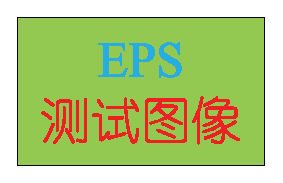
\includegraphics[width=0.3\textwidth]{chap2/testeps}}
  \hspace{1in}
  \subfigure[PDF Figure]{
    \label{fig:epspdf:b} %% label for second subfigure
    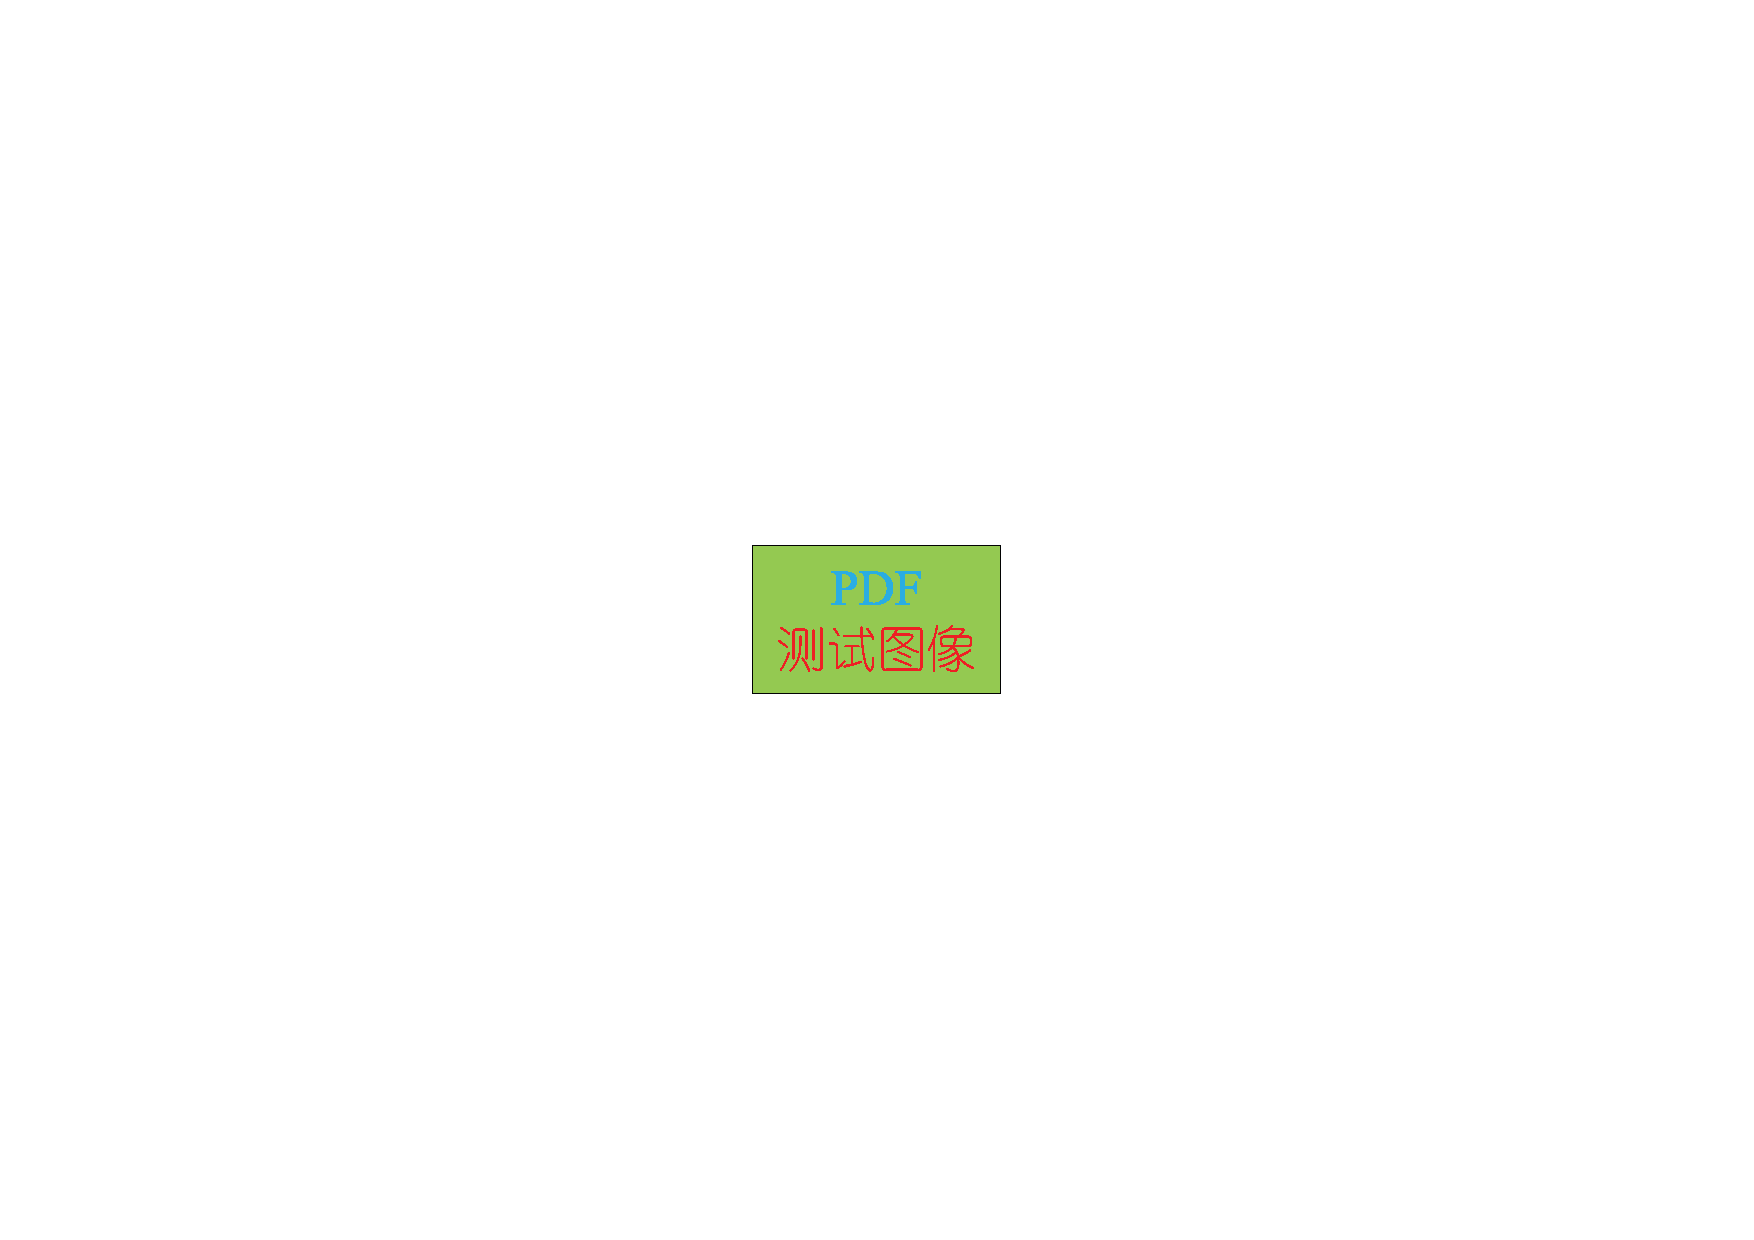
\includegraphics[angle=-90,origin=br,width=0.3\textwidth]{chap2/testpdf.pdf}}
  \bicaption[fig:pdfeps]{插入eps图像和pdf图像}{插入eps和pdf的例子}{Fig}{An EPS and PDF demo}
\end{figure}

更多关于 \LaTeX 插图的例子可以参考\href{http://www.cs.duke.edu/junhu/Graphics3.pdf}{《\LaTeX 插图指南》}。

\subsection{长标题的换行}
\label{sec:longcaption}

图\ref{fig:longcaptionbad}和图\ref{fig:longcaptiongood}都有比较长图标题,通过对比发现,图\ref{fig:longcaptiongood}的换行效果更好一些。
其中使用了minipage环境来限制整个浮动题的宽度。

\begin{figure}[!htp]
 \centering
 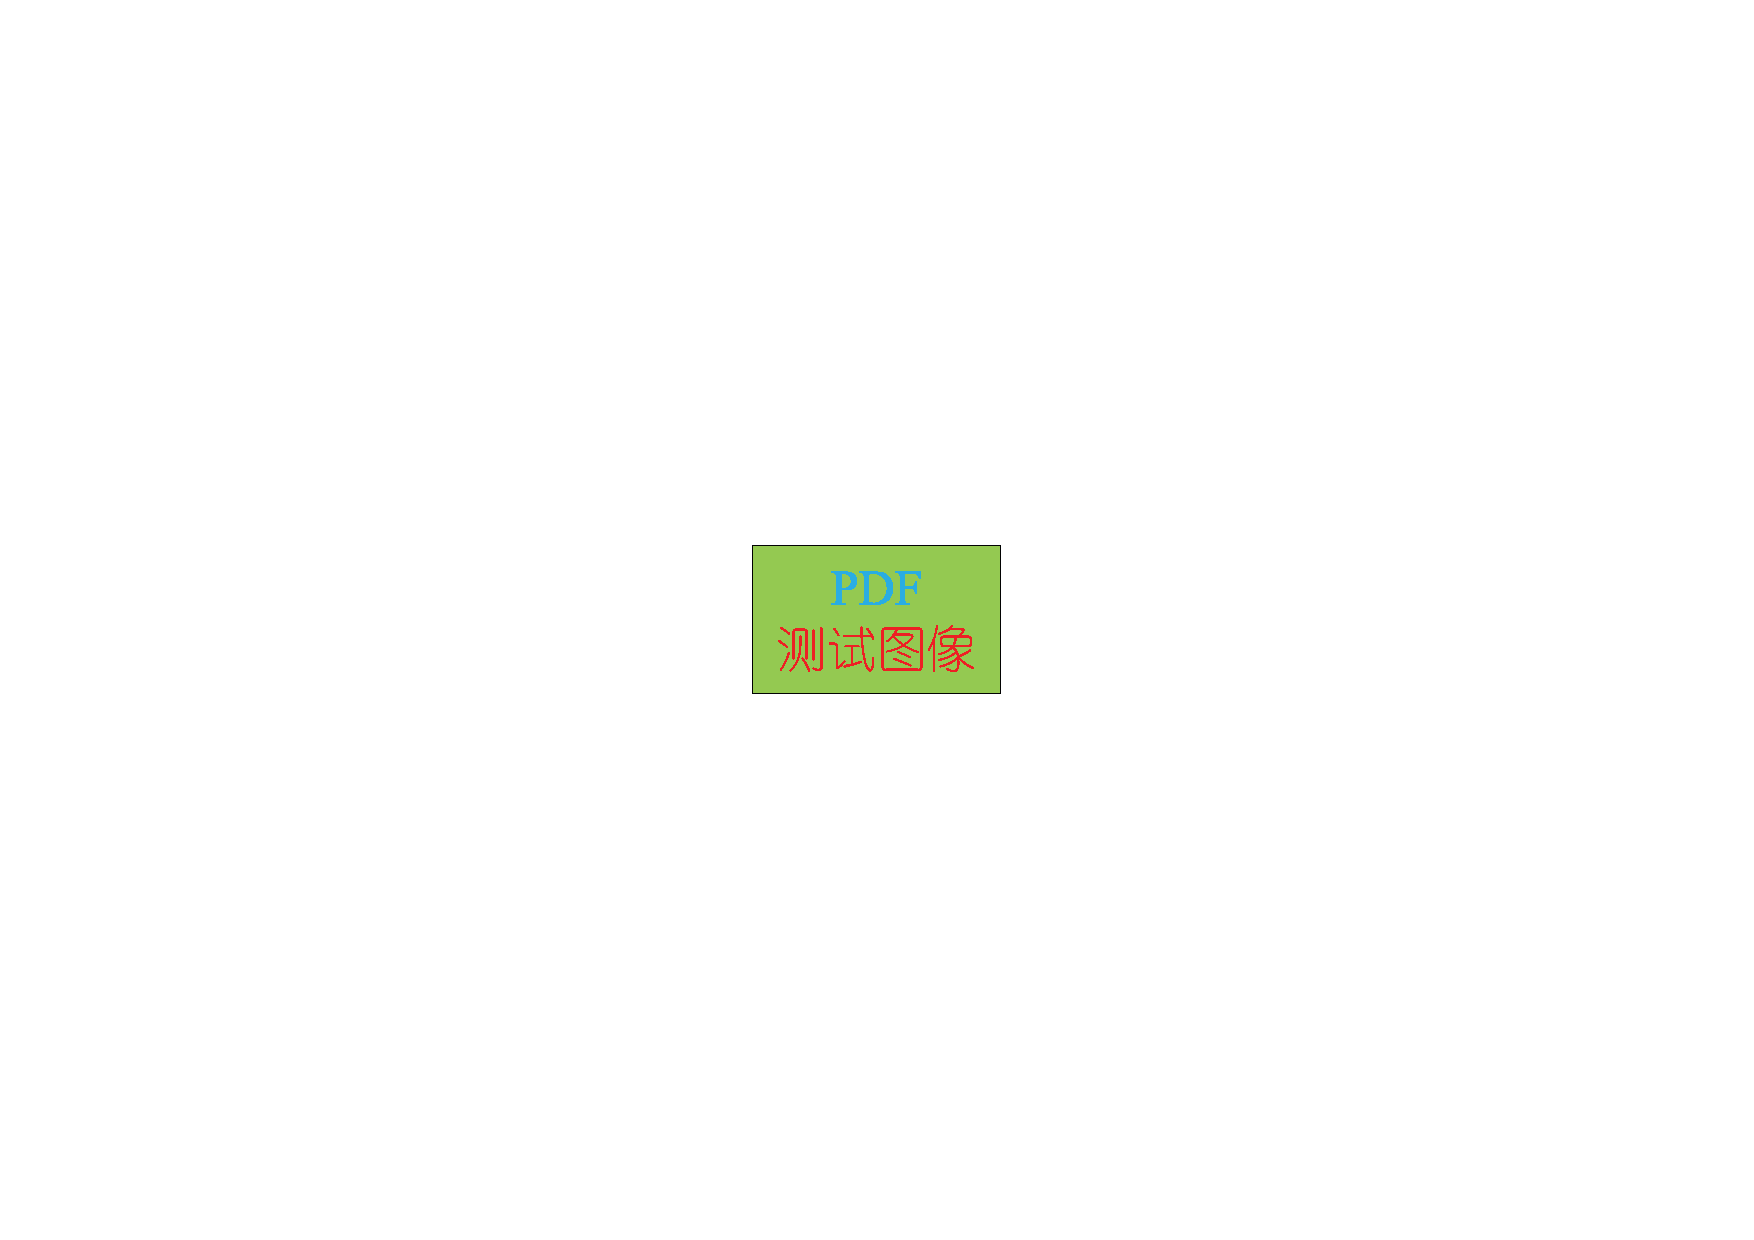
\includegraphics[angle=-90,origin=br,width=4cm]{chap2/testpdf.pdf}
 \bicaption[fig:longcaptionbad]{这里将出现在插图索引}{海交通大学是我国历史最悠久的高等学府之一,是教育部直属、教育部与上海市共建的全国重点大学.}{Fig}{Where there is a will, there is a way.}
\end{figure}


  \begin{figure}[!hbp]
    \centering
    \begin{minipage}[b]{0.6\textwidth}
      \captionstyle{\centering}
      \centering
      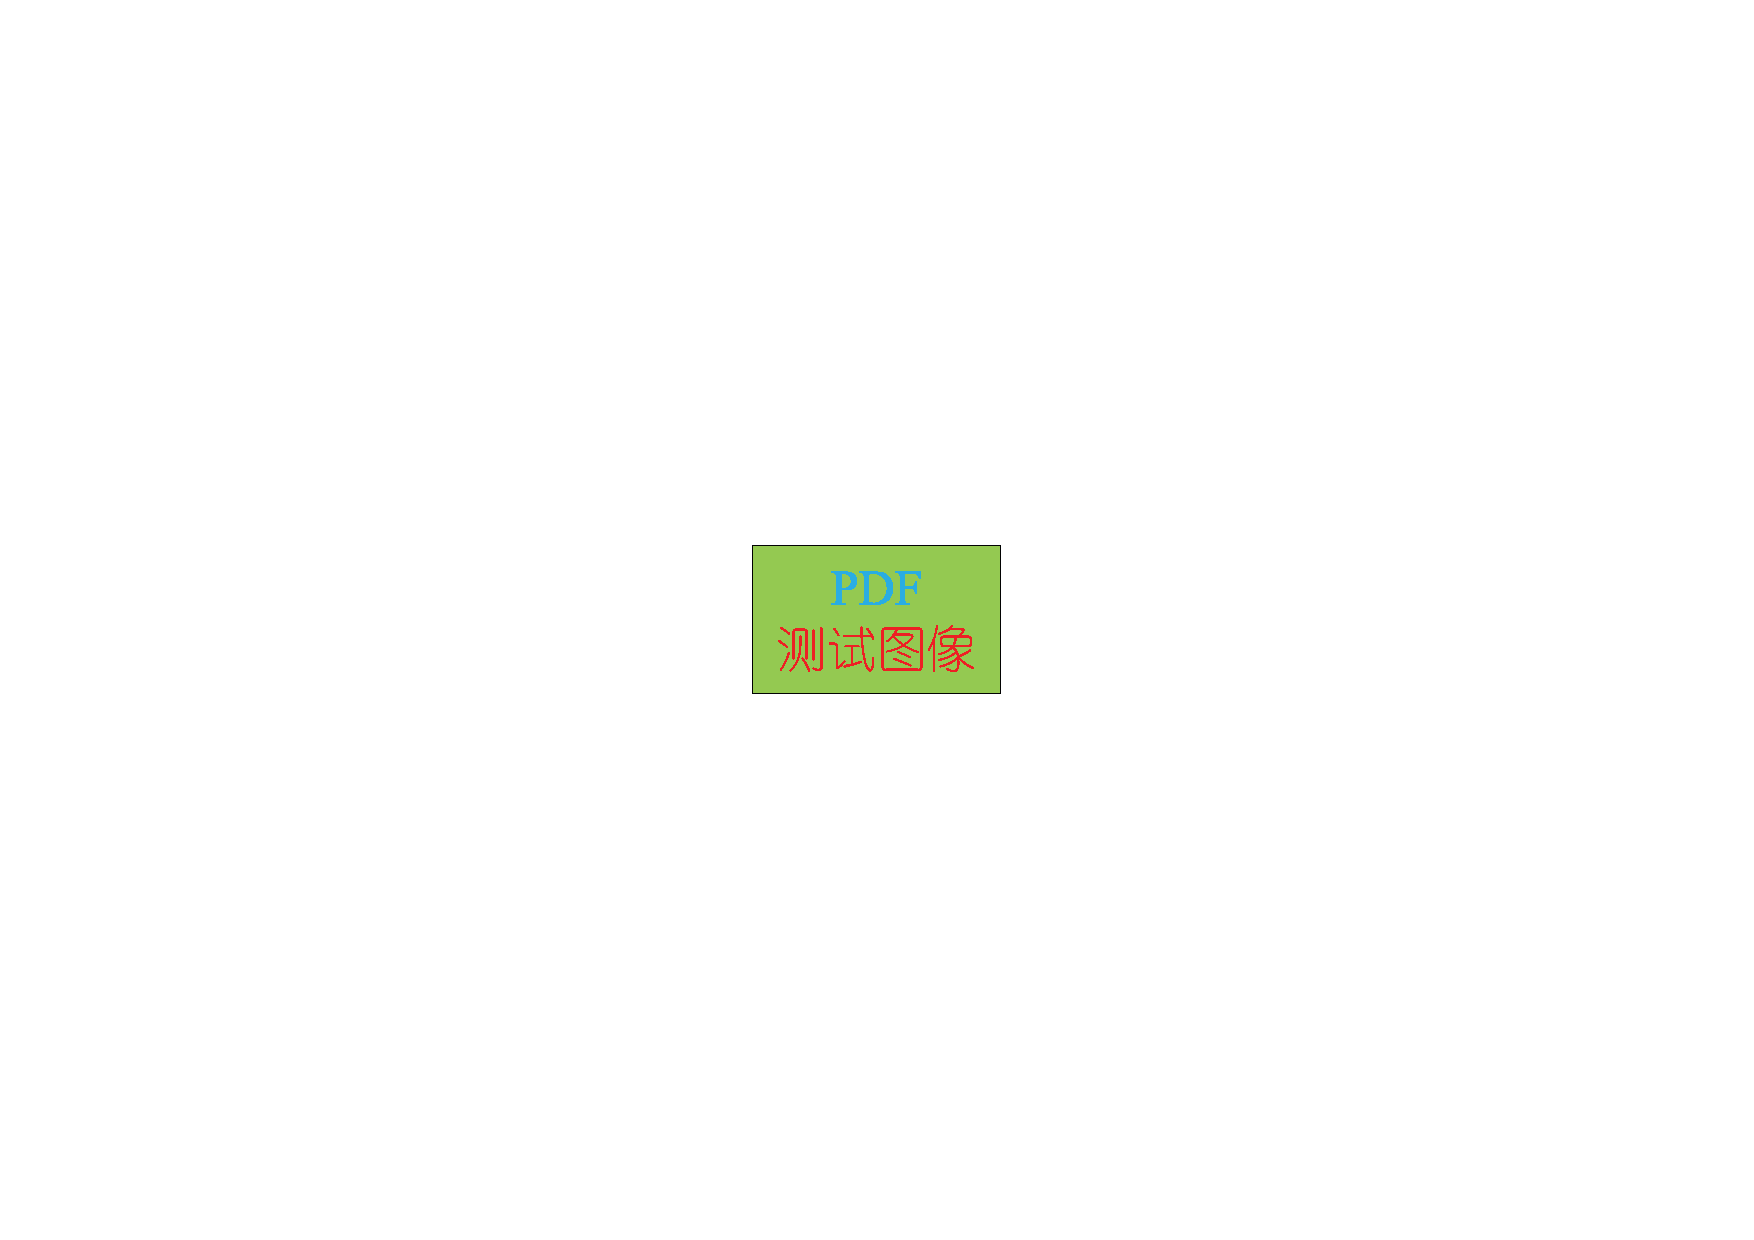
\includegraphics[angle=-90,origin=br,width=4cm]{chap2/testpdf.pdf}
      \bicaption[fig:longcaptiongood]{这里将出现在插图索引}{海交通大学是我国历史最悠久的高等学府之一,是教育部直属、教育部与上海市共建的全国重点大学.}{Fig}{Where there is a will, there is a way.}
    \end{minipage}     
  \end{figure}

  
\section{表格的例子}
\label{sec:tab}

这一节给出的是一些表格的例子,如表\ref{tab:firstone}所示。

\begin{table}[!hpb]
  \centering
  \bicaption[tab:firstone]{指向一个表格的表目录索引}{一个颇为标准的三线表格\footnotemark[1]}{Table}{A Table}
  \begin{tabular}{@{}llr@{}} \toprule
    \multicolumn{2}{c}{Item} \\ \cmidrule(r){1-2}
    Animal & Description & Price (\$)\\ \midrule
    Gnat & per gram & 13.65 \\
    & each & 0.01 \\
    Gnu & stuffed & 92.50 \\
    Emu & stuffed & 33.33 \\
    Armadillo & frozen & 8.99 \\ \bottomrule
  \end{tabular}
\end{table}
\footnotetext[1]{这个例子来自\href{http://www.ctan.org/tex-archive/macros/latex/contrib/booktabs/booktabs.pdf}{《Publication quality tables in LATEX》}(booktabs宏包的文档)。这也是一个在表格中使用脚注的例子,请留意与threeparttable实现的效果有何不同。}

下面一个是一个更复杂的表格,用threeparttable实现带有脚注的表格,如表\ref{tab:footnote}。

\begin{table}[!htpb]
  \bicaption[tab:footnote]{出现在表目录的标题}{一个带有脚注的表格的例子}{Table}{A Table with footnotes}
  \centering
  \begin{threeparttable}[b]
     \begin{tabular}{ccd{4}cccc}
      \toprule
      \multirow{2}{6mm}{total}&\multicolumn{2}{c}{20\tnote{1}} & \multicolumn{2}{c}{40} &  \multicolumn{2}{c}{60}\\
      \cmidrule(lr){2-3}\cmidrule(lr){4-5}\cmidrule(lr){6-7}
      &www & k & www & k & www & k \\
      \midrule
      &$\underset{(2.12)}{4.22}$ & 120.0140\tnote{2} & 333.15 & 0.0411 & 444.99 & 0.1387 \\
      &168.6123 & 10.86 & 255.37 & 0.0353 & 376.14 & 0.1058 \\
      &6.761    & 0.007 & 235.37 & 0.0267 & 348.66 & 0.1010 \\
      \bottomrule
    \end{tabular}
    \begin{tablenotes}
    \item [1] the first note.% or \item [a]
    \item [2] the second note.% or \item [b]
    \end{tablenotes}
  \end{threeparttable}
\end{table}

\section{参考文献管理}

参考文献的管理是这个学位论文模板又一个有趣的地方。

\subsection{将参考文献的内容与表现分离}

这个论文模板使用BibTeX处理参考文献,这又是一个``内容''与``表现形式''分离的极好例子
\footnote{当然,你也可以手动编参考文献item,直接插入文档中。}。
参考文献的``内容''就是reference文件夹下的chap\textit{xx}.bib,参考文献的元数据(名称、作者、出处等)以一定的格式保存在这些纯文本文件中。
.bib文件也可以理解为参考文献的``数据库'',正文中所有引用的参考文件条目都会从这些文件中``析出''。
控制参考文献条目``表现形式''(格式)的是.bst文件。.bst文件定义了参考文献风格,使用不同的参考文献风格能将同一个参考文献条目输出成不同的格式。
当然,一个文档只能使用一个参考文献风格。本模板使用的是国标GBT7714风格的参考文献。

BibTeX的工作过程是这样的:
BibTeX读取.aux(第一次运行latex得到的)看看你引用了什么参考文献条目,
然后到.bib中找相关条目的信息,
最后根据.bst的格式要求将参考文献条目格式化输出,写到.bbl文件中。
在运行latex将.bbl插入文档之前,你可以用文本编辑器打开它,做一些小的修改。
你会发现,.bbl的格式和你自己手动写item很相似,它已经被赋予了一定的``表现形式''。

.bib数据库中的参考文献条目可以手动编写,也可以在google的学术搜索中找到。
各大数据库\footnote{譬如SCOPUS, IEEE, OSA等。}也支持将参考文献信息导出为.bib,省时省力。
以Google学术搜索为例:进入\url{http://scholar.google.com},在``学术搜索设置''中,将``文献管理软件''设为``显示导入BibTeX''的连接,保存退出。
然后学术搜索找到文献下会有``导出到BibTeX''连接,点击后Firefox会打开新的标签页,出现类似代码\ref{googlescholar}所示的内容
\footnote{展示这些.bib条目使用了listings宏包,因为listings宏包协调中文的能力很糟糕,所以读者在查看模板的这部分源代码时会看到一些非常麻烦的东西。并且,直接将源代码的这部分内容复制到.bib中可能还会出错。我的建议是:这部分内容留意PDF就足够了。}。
请注意,这个条目离``规范''还有一些距离。

  \begin{lstlisting}[caption={从Google Scholar找到的,但并不规范的.bib条目}, label=googlescholar, float, escapeinside="", numbers=none]
    @phdthesis{"白2008信用风险传染模型和信用衍生品的定价",
      title={{"信用风险传染模型和信用衍生品的定价"}},
      author={"白云芬"},
      year={2008},
      school={"上海交通大学"}
    } 
  \end{lstlisting}

  上面的.bib条目的``名字''\cndash{}``白2008信用风险传染模型和信用衍生品的定价'',包含ASCII以外的字符,BibTeX无法处理;
  条目还缺少了address域,这样编译出来的结果会出现``地址不详'';
  并且,条目还缺少language域,BibTeX需要language域来判断是否是中文参考文献。
  将上面的条目修正(改英文名、增加address和language域),复制到本地的.bib文件中就可以了。
  显然,这里描述的是参考文献的内容,而不是表现形式。

  \begin{lstlisting}[caption={一个符合规范的.bib条目}, label=itemok, float, escapeinside="", numbers=none]
    @phdthesis{bai2008,
      title={{"信用风险传染模型和信用衍生品的定价"}},
      author={"白云芬"},
      year={2008},
      language={zh},
      address={"上海"},
      school={"上海交通大学"}
    } 
  \end{lstlisting}

由于中英文参考文献处理起来有差异,所以需要在参考文献中标注是否是中文文献。
确切地说,BibTeX并不具有区分中英文参考文献的``智能'',这种智慧的来源是.bst文——它定义了处理参考文献的规则。
GBT7714-2005NLang.bst中规定:.bib中的条目,如果条目的``language''域非空,就被认为是中文文献,否则被认为是英文文献。
例如,刚才的文献,就会被认为是中文参考文献,采取一些针对中文的处理方式。

最后,这个条目被bibtex处理后,赋予了一定的``表现形式'',在.bbl文件中以下面的样子出现。
你还可以对它进行小的修改。
再次运行latex之后,它将被插入到文档中。

\begin{lstlisting}[caption={.bbl中被格式化之后的条目}, escapeinside="", numbers=none]
\bibitem["白云芬(2008)"]{bai2008}
  \textsc{"白云芬"}.
  \newblock {"信用风险传染模型和信用衍生品的定价"}[D].
  \newblock "上海: 上海交通大学, 2008."
\end{lstlisting}

另外,
.bst文件书写起来非常繁杂\footnote{可以参考\href{http://ftp.ctex.org/mirrors/CTAN/info/bibtex/tamethebeast/ttb_en.pdf}{《Tame The BeaST》}。},书写符合GBT7714标准的.bst文件更是一项浩大的工程。
因此,当大家为漂亮、标准的参考文献列表感到满意时,应该对GBT7714-2005NLang.bst的作者充满谢意。
作者在CTeX BBS发的帖子,请看
\href{http://bbs.ctex.org/viewthread.php?tid=33571&highlight=\%B2\%CE\%BF\%BC\%CE\%C4\%CF\%D7\%2BGB}{文后参考文献著录规则 GB/T 7714-2005}。
关于GB/T 7714-2005标准本身,请看\href{http://bbs.ctex.org/viewthread.php?tid=33571&highlight=GB\%2B\%B2\%CE\%BF\%BC\%CE\%C4\%CF\%D7}{这里}。

.bib是“参考文献的内容”,而控制参考文献表现(格式)的是.bst文件,本模板附带的是GBT7714-2005NLang.bst。

\subsection{在正文中引用参考文献}

参考文献可以分章节管理,只需要在主文件中的参考文献中都包含进去就可以,如\verb+\bibliography{chap1,chap2,...}+。

正文中引用参考文献时,用\verb+\upcite{key1,key2,key3...}+可以产生“上标引用的参考文献”,
如\upcite{Meta_CN,chen2007act,DPMG}。
使用\verb+\cite{key1,key2,key3...}+则可以产生水平引用的参考文献,例如\cite{JohnD,zhubajie,IEEE-1363}。
请看下面的例子,将会穿插使用水平的和上标的参考文献:关于书的\cite{Meta_CN,JohnD,IEEE-1363},关于期刊的\upcite{chen2007act,chen2007ewi},
会议论文\cite{DPMG,kocher99,cnproceed},
硕士学位论文\cite{zhubajie,metamori2004},博士学位论文\upcite{shaheshang,FistSystem01,bai2008},标准文件\cite{IEEE-1363},技术报告\upcite{NPB2},电子文献\cite{xiaoyu2001, CHRISTINE1998},用户手册\cite{RManual}。

最后总结一些注意事项:
\begin{itemize}
\item 参考文献只有在正文中被引用了,才会在最后的参考文献列表中出现;
\item 参考文献``数据库文件''.bib是纯文本文件,请使用UTF-8编码,不要使用GBK编码;
\item 参考文献条目中通过language域是否为空判断是否是中文文献;
\item 参考文献条目同样有“内容”和“表现形式”之分,这种可控性是BibTeX带来的。
\end{itemize}


\subsection{参考文献管理器}

参考文献数据库.bib虽然是纯文本的,可以用任意的文本编辑器查看,但总有人喜欢一个找一个``可视化''地查看每一条参考文献。
我想\href{http://jabref.sourceforge.net/}{JabRef}应该是个很不错的选择。
这是一个Java写的程序,需要JRE才能运行。就测试情况来看,很幸运,JabRef可以顺利打开GBK编码的.bib文件。
但是,打开UTF--8编码的.bib源文件过程中总会崩溃,原因不得而知。
由于我们的.bib文件使用的是UTF-8编码,所以JabRef暂时不可用。

提到参考文献管理器,不得不提到另一个广被使用的软件——\href{http://www.endnote.com/}{EndNote}。
EndNote可以导入.bib文件,却不能导出.bib,只能导出.bbl——被格式化的.bib。
看来,EndNote和Word配合得更好一些。


\section{用listings插入源代码}

原先ctexbook文档类和listings宏包配合使用时,代码在换页时会出现莫名其妙的错误,后来经高人指点,顺利解决了。
感兴趣的话,可以看看\href{http://bbs.ctex.org/viewthread.php?tid=53451}{这里}。
这里给使用listings宏包插入源代码的例子,这里是一段C代码。
另外,listings宏包真可谓博大精深,可以实现各种复杂、漂亮的效果,想要进一步学习的同学,可以参考
\href{http://mirror.ctan.org/macros/latex/contrib/listings/listings.pdf}{listings宏包手册}。

\begin{lstlisting}[language={C}, caption={一段C源代码}]
#include <stdio.h>
#include <unistd.h>
#include <sys/types.h>
#include <sys/wait.h>

int main() {
  pid_t pid;

  switch ((pid = fork())) {
  case -1:
    printf("fork failed\n");
    break;
  case 0:
    /* child calls exec */
    execl("/bin/ls", "ls", "-l", (char*)0);
    printf("execl failed\n");
    break;
  default:
    /* parent uses wait to suspend execution until child finishes */
    wait((int*)0);
    printf("is completed\n");
    break;
  }

  return 0;
}
\end{lstlisting}

再给一个插入MATLAB代码的例子,感谢daisying站友提供的代码。

\begin{lstlisting}[language={matlab}, caption={一段MATLAB源代码}]
function paper1
r=0.05;
n=100;
T=1;
X=1;
v0=0.8;
sigma=sqrt(0.08);
deltat=T/n;
for i=1:n
    t(i)=i*deltat;
    w(i)=random('norm',0,t(i),1);
end
for i=1:n
    alpha(i)=0.39;
end
for i=1:n
    temp=0;
    for k=1:i
        temp=temp+alpha(k);
    end
    B(i)=exp(r*t(i));
    BB(i)=B(i)*exp(temp*deltat);
    BBB(i)=exp(-r*(T-t(i)));
end
for i=1:n
    s0(i)=X*BBB(i);
    v(i)=v0*exp((r-0.5*sigma^2)*t(i)+sigma*w(i));
    for j=i+1:n
        D=X*BBB(j);
        d1=(log(v(i)/D)+(r+sigma^2/2)*(t(j)-t(i)))/(sigma*sqrt(t(j)-t(i)));
        d2=d1-(sigma*sqrt(t(j)-t(i)));
        ppp(i,j)=D*exp(-r*(t(j)-t(i)))*(1-cdf('normal',d2,0,1))-v(i)*(1-cdf('n
ormal',d1,0,1));
    end
end
for i=1:n
    s1(i)=0;
    for j=i+1:n
        s1(i)=s1(i)+BB(j)^(-1)*alpha(j)*deltat*(X*BBB(j)-B(j)/B(i)*ppp(i,j));
    end
    s2(i)=0;
    for j=1:n
        s2(i)=s2(i)+alpha(j);
    end
    s2(i)=X*exp(-r*T-s2(i)*deltat);
    s(i)=BB(i)*(s1(i)+s2(i));
end
plot(s)
hold on;
plot(s0);
\end{lstlisting}

%%==================================================
%% chapter03.tex for SJTU Bachelor Thesis
%% version: 0.5.2
%% Encoding: UTF-8
%%==================================================

% \bibliographystyle{sjtu2} %[此处用于每章都生产参考文献]

\chapter{已知问题}
\label{chap:needsomehelp}

由于时间非常仓促,这个模板肯定存在不少问题,所以教务处希望大家帮助一起解决这些问题。下面是一些模板需要改进的地方。

\subsubsection*{这模板有点丑}
这个模板的版面设计有点不和谐,离一个“工整严谨”的科技论文模板还有一段距离,但是不知道是什么地方出了问题。欢迎来信or在BBS上指正版面设计事宜。

\subsubsection*{为什么左右页边距不一样}
如果你选的是双面打印模板,迎面页和背面页的页边距是要交换的,多出来的那一部分是留作装订的。

\subsubsection*{为什么在参考文献中会有``//''符号}
那是国标GBT7714参考文献风格规定的。

\subsubsection*{为什么参考文献中会有[s.n.],[S.l], [EB/OL]等符号}
那也是国标GBT7714参考文献风格定义的。[s.n.]表示出版者不祥,[S.l]表示出版地不祥,[EB/OL]表示引用的参考文献类型为在线电子文档。

\subsubsection*{如何获得帮助和反馈意见}
你可以通过如下的途径反馈模板使用过程中遇到的问题:\href{https://github.com/weijianwen/sjtu-thesis-template-latex/issues}{开issue}
、\href{https://bbs.sjtu.edu.cn/bbsdoc?board=TeX_LaTeX}{水源LaTeX版}发帖,或者是给\href{mailto:weijianwen@gmail.com}{Jianwen}发送邮件---你可能需要好几天才能收到邮件回复。

\subsubsection*{使用文本编辑器查看tex文件时遇到乱码}
请确保你的文本编辑器使用UTF-8编码打开了tex源文件。

\subsubsection*{在CTeX编译模板遇到``rsfs10.tfm already exists''的错误提示}
请删除\verb+X:\CTEX\UserData\fonts\tfm\public\rsfs+下的文件再重新编译。问题讨论见\href{https://bbs.sjtu.edu.cn/bbstcon,board,TeX_LaTeX,reid,1352982719.html}{水源2023号帖}。

\subsubsection*{升级了TeXLive 2012,编译后的文档出现``minus''等字样}
这是xltxtra和fontspec宏包导致的问题。学位论文模板从0.5起使用metatlog宏包代替xltxtra生成 \XeTeX 标志,解决了这个问题。

\subsubsection*{为什么在bib中加入的参考文献,没有在参考文献列表中出现?}
bib中的参考文献条目,只有通过\verb+\cite+或者\verb+\upcite+在正文中引用,才会加入到参考文献列表中。


\chapter{blabla}

%%==================================================
%% conclusion.tex for SJTU Bachelor Thesis
%% version: 0.5.2
%% Encoding: UTF-8
%%==================================================

\chapter*{全文总结\markboth{全文总结}{}}
\addcontentsline{toc}{chapter}{全文总结}

这里是全文总结内容。

 %% 全文总结


%%%%%%%%%%%%%%%%%%%%%%%%%%%%%% 
%% 附录(章节编号重新计算,使用字母进行编号)
%%%%%%%%%%%%%%%%%%%%%%%%%%%%%% 
\appendix

% 附录中编号形式是"A-1"的样子
\renewcommand\theequation{\Alph{chapter}--\arabic{equation}}
\renewcommand\thefigure{\Alph{chapter}--\arabic{figure}}
\renewcommand\thetable{\Alph{chapter}--\arabic{table}}

%%==================================================
%% app1.tex for SJTU Bachelor Thesis
%% version: 0.5.2
%% Encoding: UTF-8
%%==================================================

\chapter{模板更新记录}
\label{chap:updatelog}

\textbf{2012年12月27日} v0.5.2发布,更正拼写错误:从``个人建立''更正为``个人简历''。在diss.tex加入ack.tex,更名后忘了引用。

\textbf{2012年12月21日} v0.5.1发布,在 \LaTeX 命令和中文字符之间留了空格,在Makefile中增加release功能。

\textbf{2012年12月5日} v0.5发布,修改说明文件的措辞,更正Makefile文件,使用metalog宏包替换xltxtra宏包,使用mathtools宏包替换amsmath宏包,移除了所有CJKtilde(\verb+~+)符号。

\textbf{2012年5月30日} v0.4发布,包含交大学士、硕士、博士学位论文模板。模板在\href{https://github.com/weijianwen/sjtu-thesis-template-latex}{github}上管理和更新。

\textbf{2010年12月5日} v0.3a发布,移植到 \XeTeX/\LaTeX 上。

\textbf{2009年12月25日} v0.2a发布,模板由CASthesis改名为sjtumaster。在diss.tex中可以方便地改变正文字号、切换但双面打印。增加了不编号的一章“全文总结”。
添加了可伸缩符号(等号、箭头)的例子,增加了长标题换行的例子。

\textbf{2009年11月20日} v0.1c发布,增加了Linux下使用ctex宏包的注意事项、.bib条目的规范要求,
修正了ctexbook与listings共同使用时的断页错误。

\textbf{2009年11月13日} v0.1b发布,完善了模板使用说明,增加了定理环境、并列子图、三线表格的例子。

\textbf{2009年11月12日} 上海交通大学硕士学位论文 \LaTeX 模板发布,版本0.1a。

 % 更新记录
%% app2.tex for SJTU Bachelor Thesis
%% version: 0.5.2
%% Encoding: UTF-8
%%==================================================

\chapter{Maxwell Equations}

选择二维情况,有如下的偏振矢量
\begin{subequations}
  \begin{eqnarray}
    {\bf E}&=&E_z(r,\theta)\hat{\bf z} \\
    {\bf H}&=&H_r(r,\theta))\hat{ \bf r}+H_\theta(r,\theta)\hat{\bm
      \theta}
  \end{eqnarray}
\end{subequations}
对上式求旋度
\begin{subequations}
  \begin{eqnarray}
    \nabla\times{\bf E}&=&\frac{1}{r}\frac{\partial E_z}{\partial\theta}{\hat{\bf r}}-\frac{\partial E_z}{\partial r}{\hat{\bm\theta}}\\
    \nabla\times{\bf H}&=&\left[\frac{1}{r}\frac{\partial}{\partial
        r}(rH_\theta)-\frac{1}{r}\frac{\partial
        H_r}{\partial\theta}\right]{\hat{\bf z}}
  \end{eqnarray}
\end{subequations}
因为在柱坐标系下,$\overline{\overline\mu}$是对角的,所以Maxwell方程组中电场$\bf
E$的旋度
\begin{subequations}
  \begin{eqnarray}
    &&\nabla\times{\bf E}=\mathbf{i}\omega{\bf B} \\
    &&\frac{1}{r}\frac{\partial E_z}{\partial\theta}{\hat{\bf
        r}}-\frac{\partial E_z}{\partial
      r}{\hat{\bm\theta}}=\mathbf{i}\omega\mu_rH_r{\hat{\bf r}}+\mathbf{i}\omega\mu_\theta
    H_\theta{\hat{\bm\theta}}
  \end{eqnarray}
\end{subequations}
所以$\bf H$的各个分量可以写为:
\begin{subequations}
  \begin{eqnarray}
    H_r=\frac{1}{\mathbf{i}\omega\mu_r}\frac{1}{r}\frac{\partial
      E_z}{\partial\theta } \\
    H_\theta=-\frac{1}{\mathbf{i}\omega\mu_\theta}\frac{\partial E_z}{\partial r}
  \end{eqnarray}
\end{subequations}
同样地,在柱坐标系下,$\overline{\overline\epsilon}$是对角的,所以Maxwell方程组中磁场$\bf
H$的旋度
\begin{subequations}
  \begin{eqnarray}
    &&\nabla\times{\bf H}=-\mathbf{i}\omega{\bf D}\\
    &&\left[\frac{1}{r}\frac{\partial}{\partial
        r}(rH_\theta)-\frac{1}{r}\frac{\partial
        H_r}{\partial\theta}\right]{\hat{\bf
        z}}=-\mathbf{i}\omega{\overline{\overline\epsilon}}{\bf
      E}=-\mathbf{i}\omega\epsilon_zE_z{\hat{\bf z}} \\
    &&\frac{1}{r}\frac{\partial}{\partial
      r}(rH_\theta)-\frac{1}{r}\frac{\partial
      H_r}{\partial\theta}=-\mathbf{i}\omega\epsilon_zE_z
  \end{eqnarray}
\end{subequations}
由此我们可以得到关于$E_z$的波函数方程:
\begin{eqnarray}
  \frac{1}{\mu_\theta\epsilon_z}\frac{1}{r}\frac{\partial}{\partial r}
  \left(r\frac{\partial E_z}{\partial r}\right)+
  \frac{1}{\mu_r\epsilon_z}\frac{1}{r^2}\frac{\partial^2E_z}{\partial\theta^2}
  +\omega^2 E_z=0
\end{eqnarray}
 % 麦克斯韦方程
% \include{body/app3}


%%%%%%%%%%%%%%%%%%%%%%%%%%%%%% 
%% 文后(无章节编号)
%%%%%%%%%%%%%%%%%%%%%%%%%%%%%% 
\backmatter

% 参考文献
% 使用 BibTeX
% 包含参考文献文件.bib
\bibliography{reference/chap1,reference/chap2}

%% 个人简历(学士学位论文没有个人简历要求)
% %%==================================================
%% resume.tex for SJTU Bachelor Thesis
%% version: 0.5.2
%% Encoding: UTF-8
%%==================================================

\begin{resume}

\begin{resumesection}{基本情况}
xxx,男,上海人,19XX 年~XX 月出生,未婚,
上海交通大学XX系在读。
\end{resumesection}

\begin{resumelist}{教育状况}
XXXX 年~9 月至~XXXX 年~7 月,上海交通大学, 本科,专业:XXXX

XXXX 年~9 月至~XXXX 年~7 月,上海交通大学, 硕士研究生,专业:XXXX

XXXX 年~9 月至~XXXX 年~7 月,上海交通大学,
博士研究生(提前攻读博士),专业:XXXX
\end{resumelist}

\begin{resumelist}{工作经历}
无。
\end{resumelist}

\begin{resumelist}{研究兴趣}
XXXXXXX。
\end{resumelist}

\begin{resumelist}{联系方式}
通讯地址:上海市闵行区东川路800号,上海交通大学

邮编:200240

E-mail: abcde@sjtu.edu.cn
\end{resumelist}

\end{resume}


% 致谢
%%==================================================
%% thanks.tex for SJTU Bachelor Thesis
%% version: 0.5.2
%% Encoding: UTF-8
%%==================================================

\begin{thanks}

在本课题的进展以及本文的撰写过程中,包括导师伍民友以及王新兵老师在内的一些老师和很多同学们都给了我非常多的支持和帮助,我要再次表达对你们的感谢.

首先是我的论文导师伍民友老师,以及一同指导我的王新兵老师.他们在本课题从开始的决定课题内容一直到最后课题的完成,再到论文的写作过程,都以严格的标准要求我,每周都会主动地找我进行交流,了解课题的进展情况.除此之外,他们也为课题的进展直到完成提出了许多非常宝贵的意见和指导.

其次我要感谢王新兵老师的物联网实验室,不仅提供了本文中所使用的大量的学术论文数据,还提供了配置精良的机器以供我的课题作为计算资源.这极大的加快了我的开发进度,缩短了我对于课题中遇到的问题所需要的对应的时间,是我课题能够顺利完成的关键之一.

最后我要感谢学校和学院为我课题的完成提供了如此优良的环境.学校提供的学术资源数据库以及科研条件让我在研究过程中没有遇到什么课题以外的障碍,让课题得以顺利完成.


\end{thanks}



% 发表文章目录
%%%==================================================
%% pub.tex for SJTU Bachelor Thesis
%% version: 0.5.2
%% Encoding: UTF-8
%%==================================================

\begin{publications}{99}

    \item\textsc{Chen H, Chan C~T}. {Acoustic cloaking in three dimensions using acoustic metamaterials}[J].
      Applied Physics Letters, 2007, 91:183518.

    \item\textsc{Chen H, Wu B~I, Zhang B}, et al. {Electromagnetic Wave Interactions with a Metamaterial Cloak}[J].
      Physical Review Letters, 2007, 99(6):63903.
    
\end{publications}


% 参与项目列表
%%%==================================================
%% projects.tex for SJTU Bachelor Thesis
%% version: 0.5.2
%% Encoding: UTF-8
%%==================================================

\begin{projects}{99}

    \item 973项目“XXX”
    \item 自然基金项目“XXX”
    \item 国防项目“XXX”
    
\end{projects}


%英文大摘要
%%==================================================
%% bigabstract.tex for SJTU Bachelor Thesis
%% version: 0.5.2
%% Encoding: UTF-8
%%==================================================

\begin{bigabstract}

An imperial edict issued in 1896 by Emperor Guangxu, established Nanyang Public School in Shanghai. The normal school, school of foreign studies, middle school and a high school were established. Sheng Xuanhuai, the person responsible for proposing the idea to the emperor, became the first president and is regarded as the founder of the university.

During the 1930s, the university gained a reputation of nurturing top engineers. After the foundation of People's Republic, some faculties were transferred to other universities. A significant amount of its faculty were sent in 1956, by the national government, to Xi'an to help build up Xi'an Jiao Tong University in western China. Afterwards, the school was officially renamed Shanghai Jiao Tong University.

Since the reform and opening up policy in China, SJTU has taken the lead in management reform of institutions for higher education, regaining its vigor and vitality with an unprecedented momentum of growth. SJTU includes five beautiful campuses, Xuhui, Minhang, Luwan Qibao, and Fahua, taking up an area of about 3,225,833 m2. A number of disciplines have been advancing towards the top echelon internationally, and a batch of burgeoning branches of learning have taken an important position domestically.

Today SJTU has 31 schools (departments), 63 undergraduate programs, 250 masters-degree programs, 203 Ph.D. programs, 28 post-doctorate programs, and 11 state key laboratories and national engineering research centers.

SJTU boasts a large number of famous scientists and professors, including 35 academics of the Academy of Sciences and Academy of Engineering, 95 accredited professors and chair professors of the "Cheung Kong Scholars Program" and more than 2,000 professors and associate professors.

Its total enrollment of students amounts to 35,929, of which 1,564 are international students. There are 16,802 undergraduates, and 17,563 masters and Ph.D. candidates. After more than a century of operation, Jiao Tong University has inherited the old tradition of "high starting points, solid foundation, strict requirements and extensive practice." Students from SJTU have won top prizes in various competitions, including ACM International Collegiate Programming Contest, International Mathematical Contest in Modeling and Electronics Design Contests. Famous alumni include Jiang Zemin, Lu Dingyi, Ding Guangen, Wang Daohan, Qian Xuesen, Wu Wenjun, Zou Taofen, Mao Yisheng, Cai Er, Huang Yanpei, Shao Lizi, Wang An and many more. More than 200 of the academics of the Chinese Academy of Sciences and Chinese Academy of Engineering are alumni of Jiao Tong University.

\end{bigabstract}


\end{document}
